\documentclass{extbook}[14pt]
\usepackage{multicol, enumerate, enumitem, hyperref, color, soul, setspace, parskip, fancyhdr, amssymb, amsthm, amsmath, bbm, latexsym, units, mathtools}
\everymath{\displaystyle}
\usepackage[headsep=0.5cm,headheight=0cm, left=1 in,right= 1 in,top= 1 in,bottom= 1 in]{geometry}
\usepackage{dashrule}  % Package to use the command below to create lines between items
\newcommand{\litem}[1]{\item #1

\rule{\textwidth}{0.4pt}}
\pagestyle{fancy}
\lhead{}
\chead{Answer Key for Progress Quiz 4 Version A}
\rhead{}
\lfoot{9187-5854}
\cfoot{}
\rfoot{Spring 2021}
\begin{document}
\textbf{This key should allow you to understand why you choose the option you did (beyond just getting a question right or wrong). \href{https://xronos.clas.ufl.edu/mac1105spring2020/courseDescriptionAndMisc/Exams/LearningFromResults}{More instructions on how to use this key can be found here}.}

\textbf{If you have a suggestion to make the keys better, \href{https://forms.gle/CZkbZmPbC9XALEE88}{please fill out the short survey here}.}

\textit{Note: This key is auto-generated and may contain issues and/or errors. The keys are reviewed after each exam to ensure grading is done accurately. If there are issues (like duplicate options), they are noted in the offline gradebook. The keys are a work-in-progress to give students as many resources to improve as possible.}

\rule{\textwidth}{0.4pt}

\begin{enumerate}\litem{
Find the equation of the line described below. Write the linear equation as $ y=mx+b $ and choose the intervals that contain $m$ and $b$.
\[ \text{Parallel to } 9 x - 5 y = 14 \text{ and passing through the point } (-2, -4). \]The solution is \( y = 1.80x - 0.40 \), which is option D.\begin{enumerate}[label=\Alph*.]
\item \( m \in [1.4, 2.1] \hspace*{3mm} b \in [-2.97, -1.69] \)

 $y = 1.80x - 2.00$, which corresponds to correct slope and mis-distributing while simplifying to slope-intercept form.
\item \( m \in [-2.9, -0.8] \hspace*{3mm} b \in [-8.65, -6.65] \)

 $y = -1.80x - 7.60$, which corresponds to using the negative slope.
\item \( m \in [0.3, 1.1] \hspace*{3mm} b \in [-0.69, 0.25] \)

 $y = 0.56x - 0.40$, which corresponds to using the reciprocal slope $(1/m)$.
\item \( m \in [1.4, 2.1] \hspace*{3mm} b \in [-0.69, 0.25] \)

* $y = 1.80x - 0.40$, which is the correct option.
\item \( m \in [1.4, 2.1] \hspace*{3mm} b \in [0.17, 1.08] \)

 $y = 1.80x + 0.40$, which corresponds to using the correct slope and getting the negative $y$-intercept.
\end{enumerate}

\textbf{General Comment:} Parallel slope is the same and perpendicular slope is opposite reciprocal. Opposite reciprocal means flipping the fraction and changing the sign (positive to negative or negative to positive).
}
\litem{
First, find the equation of the line containing the two points below. Then, write the equation as $ y=mx+b $ and choose the intervals that contain $m$ and $b$.
\[ (4, -10) \text{ and } (8, 5) \]The solution is \( y = 3.75x -25.0 \), which is option D.\begin{enumerate}[label=\Alph*.]
\item \( m \in [0.75, 7.75] \hspace*{3mm} b \in [-5, 3] \)

 $y = 3.75x -3$, which corresponds to using the correct slope/equation but not distributing correctly using the second point.
\item \( m \in [0.75, 7.75] \hspace*{3mm} b \in [19, 31] \)

 $y = 3.75x + 25.0$, which corresponds to using the correct slope and getting the negative y-intercept.
\item \( m \in [-3.75, -2.75] \hspace*{3mm} b \in [34, 36] \)

 $y = -3.75x + 35.0$, which corresponds to using the negative slope and the correct equation.
\item \( m \in [0.75, 7.75] \hspace*{3mm} b \in [-26, -21] \)

* $y = 3.75x -25.0$, which is the correct option.
\item \( m \in [0.75, 7.75] \hspace*{3mm} b \in [-15, -13] \)

 $y = 3.75x -14$, which corresponds to using the correct slope/equation but not distributing correctly using the first point.
\end{enumerate}

\textbf{General Comment:} Remember to keep your points in order when plugging in to the slope formula.
}
\litem{
Find the equation of the line described below. Write the linear equation as $ y=mx+b $ and choose the intervals that contain $m$ and $b$.
\[ \text{Parallel to } 3 x + 5 y = 15 \text{ and passing through the point } (10, 3). \]The solution is \( y = -0.60x + 9.00 \), which is option C.\begin{enumerate}[label=\Alph*.]
\item \( m \in [-0.91, -0.12] \hspace*{3mm} b \in [-8.7, -6.3] \)

 $y = -0.60x - 7.00$, which corresponds to correct slope and mis-distributing while simplifying to slope-intercept form.
\item \( m \in [-0.91, -0.12] \hspace*{3mm} b \in [-11.6, -8.1] \)

 $y = -0.60x - 9.00$, which corresponds to using the correct slope and getting the negative $y$-intercept.
\item \( m \in [-0.91, -0.12] \hspace*{3mm} b \in [8.8, 9.2] \)

* $y = -0.60x + 9.00$, which is the correct option.
\item \( m \in [-1.72, -0.61] \hspace*{3mm} b \in [8.8, 9.2] \)

 $y = -1.67x + 9.00$, which corresponds to using the reciprocal slope $(1/m)$.
\item \( m \in [0.26, 1.97] \hspace*{3mm} b \in [-3.4, -2.1] \)

 $y = 0.60x - 3.00$, which corresponds to using the negative slope.
\end{enumerate}

\textbf{General Comment:} Parallel slope is the same and perpendicular slope is opposite reciprocal. Opposite reciprocal means flipping the fraction and changing the sign (positive to negative or negative to positive).
}
\litem{
Write the equation of the line in the graph below in Standard form $Ax+By=C$. Then, choose the intervals that contain $A, B, \text{ and } C$.

\begin{center}
    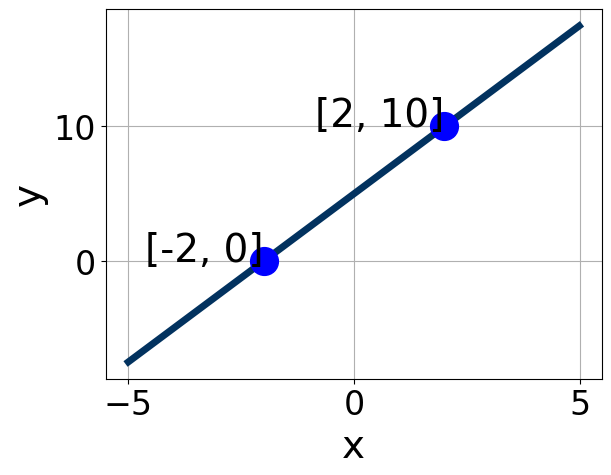
\includegraphics[width=0.5\textwidth]{../Figures/linearGraphToStandardCopyA.png}
\end{center}


The solution is \( 5x - 2y = -10 \), which is option D.\begin{enumerate}[label=\Alph*.]
\item \( A \in [-5.1, -4.2], \hspace{3mm} B \in [1.65, 2.49], \text{ and } \hspace{3mm} C \in [10, 12] \)

 $-5x + 2y = 10$, which corresponds to not making $A$ positive (by multiplying the equation by $-1$).
\item \( A \in [3.9, 7.3], \hspace{3mm} B \in [1.65, 2.49], \text{ and } \hspace{3mm} C \in [10, 12] \)

 $5x + 2y = 10$, which corresponds to using the opposite (negative) slope of the graph, but did everything else correctly.
\item \( A \in [-3.1, -0.2], \hspace{3mm} B \in [0.93, 1.23], \text{ and } \hspace{3mm} C \in [1, 6] \)

 $-2.5x + 1y = 5.0$, which corresponds to not removing rational values for Standard Form.
\item \( A \in [3.9, 7.3], \hspace{3mm} B \in [-2.14, -1.8], \text{ and } \hspace{3mm} C \in [-11, -6] \)

* $5x - 2y = -10$, which is the correct option.
\item \( A \in [-3.1, -0.2], \hspace{3mm} B \in [-1.38, -0.9], \text{ and } \hspace{3mm} C \in [-8, -3] \)

 $-2.5x - 1y = -5.0$, which corresponds to using the opposite (negative) slope of the graph and not removing rational values.
\end{enumerate}

\textbf{General Comment:} Standard form is supposed to have $A > 0$ and all fractions removed.
}
\litem{
Write the equation of the line in the graph below in Standard form $Ax+By=C$. Then, choose the intervals that contain $A, B, \text{ and } C$.

\begin{center}
    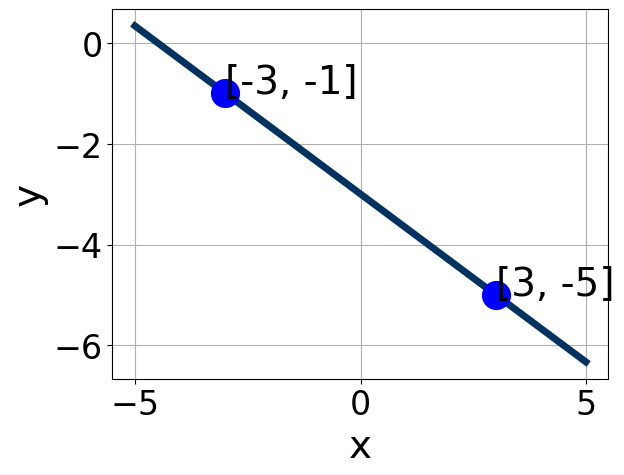
\includegraphics[width=0.5\textwidth]{../Figures/linearGraphToStandardA.png}
\end{center}


The solution is \( 5x - 4y = -8 \), which is option C.\begin{enumerate}[label=\Alph*.]
\item \( A \in [-1.25, 0.75], \hspace{3mm} B \in [-3.9, -0.6], \text{ and } \hspace{3mm} C \in [-3, 1] \)

 $-1.25x - 1y = -2.0$, which corresponds to using the opposite (negative) slope of the graph and not removing rational values.
\item \( A \in [-1.25, 0.75], \hspace{3mm} B \in [0, 3.3], \text{ and } \hspace{3mm} C \in [1, 6] \)

 $-1.25x + 1y = 2.0$, which corresponds to not removing rational values for Standard Form.
\item \( A \in [3, 7], \hspace{3mm} B \in [-5.5, -3], \text{ and } \hspace{3mm} C \in [-14, -7] \)

* $5x - 4y = -8$, which is the correct option.
\item \( A \in [-13, -4], \hspace{3mm} B \in [1.5, 6.4], \text{ and } \hspace{3mm} C \in [4, 13] \)

 $-5x + 4y = 8$, which corresponds to not making $A$ positive (by multiplying the equation by $-1$).
\item \( A \in [3, 7], \hspace{3mm} B \in [1.5, 6.4], \text{ and } \hspace{3mm} C \in [4, 13] \)

 $5x + 4y = 8$, which corresponds to using the opposite (negative) slope of the graph, but did everything else correctly.
\end{enumerate}

\textbf{General Comment:} Standard form is supposed to have $A > 0$ and all fractions removed.
}
\litem{
Solve the equation below. Then, choose the interval that contains the solution.
\[ -8(18x -11) = -2(-10x + 15) \]The solution is \( x = 0.720 \), which is option B.\begin{enumerate}[label=\Alph*.]
\item \( x \in [0.43, 0.57] \)

$x = 0.468$, which corresponds to getting the negative of the actual solution.
\item \( x \in [0.69, 0.81] \)

* $x = 0.720$, which is the correct option.
\item \( x \in [-0.44, -0.24] \)

$x = -0.354$, which corresponds to not distributing the negative in front of the first parentheses correctly.
\item \( x \in [0.33, 0.45] \)

$x = 0.354$, which corresponds to not distributing the negative in front of the second parentheses correctly.
\item \( \text{There are no real solutions.} \)

Corresponds to students thinking a fraction means there is no solution to the equation.
\end{enumerate}

\textbf{General Comment:} The most common mistake on this question is to not distribute the negative in front of the second fraction correctly. The best way to avoid this is putting the numerator in parentheses, which will help you remember to distribute the negative correctly.
}
\litem{
Solve the linear equation below. Then, choose the interval that contains the solution.
\[ \frac{5x -3}{8} - \frac{7x + 9}{2} = \frac{-9x + 8}{4} \]The solution is \( x = -11.000 \), which is option B.\begin{enumerate}[label=\Alph*.]
\item \( x \in [0.3, 1] \)

 $x = 0.982$, which corresponds to dividing the second number in the numerator by the denominator rather than dividing BOTH parts of the numerator by the denominator (or removing the fractions through multiplication).
\item \( x \in [-11.4, -10] \)

* $x = -11.000$, which is the correct option.
\item \( x \in [-33.1, -30.2] \)

 $x = -32.000$, which corresponds to dividing the coefficients in front of x by the denominator rather than dividing BOTH parts of the numerator by the denominator (or removing the fractions through multiplication).
\item \( x \in [2.4, 4.3] \)

 $x = 3.400$, which corresponds to not distributing the negative in front of the second fraction.
\item \( \text{There are no real solutions.} \)

Corresponds to students thinking a fraction means there is no solution to the equation.
\end{enumerate}

\textbf{General Comment:} If you are having trouble with this problem, try to remove a fraction at a time by multiplying each term by the denominator.
}
\litem{
Solve the equation below. Then, choose the interval that contains the solution.
\[ -12(19x + 17) = -16(-11x -4) \]The solution is \( x = -0.663 \), which is option A.\begin{enumerate}[label=\Alph*.]
\item \( x \in [-0.76, -0.4] \)

* $x = -0.663$, which is the correct option.
\item \( x \in [-0.32, 0.56] \)

$x = 0.347$, which corresponds to not distributing the negative in front of the first parentheses correctly.
\item \( x \in [-2.89, -1.82] \)

$x = -2.692$, which corresponds to getting the negative of the actual solution.
\item \( x \in [-0.47, -0.29] \)

$x = -0.347$, which corresponds to not distributing the negative in front of the second parentheses correctly.
\item \( \text{There are no real solutions.} \)

Corresponds to students thinking a fraction means there is no solution to the equation.
\end{enumerate}

\textbf{General Comment:} The most common mistake on this question is to not distribute the negative in front of the second fraction correctly. The best way to avoid this is putting the numerator in parentheses, which will help you remember to distribute the negative correctly.
}
\litem{
Solve the linear equation below. Then, choose the interval that contains the solution.
\[ \frac{4x -5}{6} - \frac{7x + 7}{3} = \frac{-7x -3}{4} \]The solution is \( x = 29.000 \), which is option D.\begin{enumerate}[label=\Alph*.]
\item \( x \in [-30, -26] \)

 $x = -27.000$, which corresponds to not distributing the negative in front of the second fraction.
\item \( x \in [-2.4, 4.6] \)

 $x = 0.604$, which corresponds to dividing the second number in the numerator by the denominator rather than dividing BOTH parts of the numerator by the denominator (or removing the fractions through multiplication).
\item \( x \in [108, 110] \)

 $x = 108.000$, which corresponds to dividing the coefficients in front of x by the denominator rather than dividing BOTH parts of the numerator by the denominator (or removing the fractions through multiplication).
\item \( x \in [29, 32] \)

* $x = 29.000$, which is the correct option.
\item \( \text{There are no real solutions.} \)

Corresponds to students thinking a fraction means there is no solution to the equation.
\end{enumerate}

\textbf{General Comment:} If you are having trouble with this problem, try to remove a fraction at a time by multiplying each term by the denominator.
}
\litem{
First, find the equation of the line containing the two points below. Then, write the equation as $ y=mx+b $ and choose the intervals that contain $m$ and $b$.
\[ (-3, 4) \text{ and } (4, -8) \]The solution is \( y = -1.71x -1.14 \), which is option B.\begin{enumerate}[label=\Alph*.]
\item \( m \in [-3, -0.6] \hspace*{3mm} b \in [0.6, 4.3] \)

 $y = -1.71x + 1.14$, which corresponds to using the correct slope and getting the negative y-intercept.
\item \( m \in [-3, -0.6] \hspace*{3mm} b \in [-1.7, 1] \)

* $y = -1.71x -1.14$, which is the correct option.
\item \( m \in [-3, -0.6] \hspace*{3mm} b \in [-13.3, -9.7] \)

 $y = -1.71x -12$, which corresponds to using the correct slope/equation but not distributing correctly using the second point.
\item \( m \in [-3, -0.6] \hspace*{3mm} b \in [6.2, 8.9] \)

 $y = -1.71x + 7$, which corresponds to using the correct slope/equation but not distributing correctly using the first point.
\item \( m \in [0, 3.2] \hspace*{3mm} b \in [-15.1, -14.8] \)

 $y = 1.71x -14.86$, which corresponds to using the negative slope and the correct equation.
\end{enumerate}

\textbf{General Comment:} Remember to keep your points in order when plugging in to the slope formula.
}
\end{enumerate}

\end{document}